\documentclass[letterpaper,11pt,oneside,reqno]{article}

%%%%%%%%%%%%%%%%%%%%%%%%%%%%%%%%%%%%%%%%%%%%%%%%%%%%%%%%%%%%

\usepackage[pdftex,backref=page,colorlinks=true,linkcolor=blue,citecolor=red]{hyperref}
\usepackage[alphabetic,nobysame]{amsrefs}

%%%%%%%%%%%%%%%%%%%%%%%%%%%%%%%%%%%%%%%%%%%%%%%%%%%%%%%%%%%%
%main packages
\usepackage{amsmath,amssymb,amsthm,amsfonts,mathtools}
\usepackage{graphicx,color}
\usepackage{upgreek}
\usepackage[mathscr]{euscript}

%equations
\allowdisplaybreaks
\numberwithin{equation}{section}
%tikz
\usepackage{tikz}

%conveniences
\usepackage{array}
\usepackage{adjustbox}
\usepackage{cleveref}
\usepackage{enumerate}
\usepackage{datetime}

%paper geometry
\usepackage[DIV=12]{typearea}

%%%%%%%%%%%%%%%%%%%%%%%%%%%%%%%%%%%%%%%%%%%%%%%%%%%%%%%%%%%%
%draft-specific
\synctex=1
% \usepackage{refcheck,comment}

%%%%%%%%%%%%%%%%%%%%%%%%%%%%%%%%%%%%%%%%%%%%%%%%%%%%%%%%%%%%
%this paper specific
\newcommand{\ssp}{\hspace{1pt}}

%%%%%%%%%%%%%%%%%%%%%%%%%%%%%%%%%%%%%%%%%%%%%%%%%%%%%%%%%%%%
\newtheorem{proposition}{Proposition}[section]
\newtheorem{lemma}[proposition]{Lemma}
\newtheorem{corollary}[proposition]{Corollary}
\newtheorem{theorem}[proposition]{Theorem}
%%%%%%%%%%%%%%%%%%%%%%%%%%%%%%%%%%%%%%%%%%%%%%%%%%%%%%%%%%%%
\theoremstyle{definition}
\newtheorem{definition}[proposition]{Definition}
\newtheorem{remark}[proposition]{Remark}
\newtheorem{example}[proposition]{Example}
%%%%%%%%%%%%%%%%%%%%%%%%%%%%%%%%%%%%%%%%%%%%%%%%%%%%%%%%%%%%

\begin{document}
\title{How to Solve the Stochastic Six Vertex Model}

% OTHER AUTHORS 

% \author{Matthew Nicoletti and Leonid Petrov}
\author{Leonid Petrov}

\date{At \currenttime{}, on \today}

\setcounter{tocdepth}{4}

\maketitle


\section*{Introduction}

These are lecture notes for \href{https://www.math.tamu.edu/conferences/functional_analysis/PANEM.html}{\texttt{PANEM-2023}} at Texas A{}\&M on the integrability and asymptotics of the stochastic six vertex model.



\newpage
\section{Six vertex model through different lenses}

In the first lecture, we describe the stochastic six vertex model
from two diverse perspectives --- as a model of statistical mechanics,
and as a stochastic particle system.

\subsection{Gibbs measures and the six vertex model}
\label{sub:gibbs_6v}

\subsubsection{Finite-volume Gibbs measures}

We begin with describing the useful framework of \emph{Gibbs measures}.
For simplicity, we work on the two-dimensional lattice $\mathbb{Z}^2$.
Let $\Lambda\subset\mathbb{Z}^{2}$ be a finite subset (for example, a rectangle).
We are interested in \emph{spin configurations} inside $\Lambda$
which are encoded as $\omega=\{\sigma_e\colon e \textnormal{ is an edge in $\Lambda$}\}$,
where $\sigma_e\in\left\{ 0,1 \right\}$.
By an ``edge in $\Lambda$'' we mean that both endpoints of this edge must be inside $\Lambda$.
Each spin configuration is equipped with boundary conditions,
which are fixed spins on all the boundary edges of $\Lambda$
(an edge is called boundary if it connects $\Lambda$ to $\mathbb{Z}^{2}\setminus \Lambda$).

With each spin configuration $\omega$, we associate 
its energy
$H(\omega)\in \mathbb{R}$.
This energy
may depend on global parameters
(e.g., inverse temperature)
and local parameters (e.g., edge capacities or vertex rapidities).
If a particular spin configuration $\omega$ is forbidden, we have $H(\omega)=+\infty$.

\begin{definition}
	\label{def:Gibbs_measure_finite}
	A (finite-volume) \emph{Gibbs measure}
	in $\Lambda$ 
	with fixed boundary conditions 
	and the energy function $H(\cdot)$
	is the probability distribution on spin configurations 
	whose probability weights have the form
	\begin{equation*}
		\mathop{\mathrm{{Prob}}}(\omega)=\frac{1}{Z}\ssp\exp\left\{ -H(\omega) \right\}.
	\end{equation*}
	Here $Z$ is the \emph{partition function}, which is simply the probability normalizing constant.
\end{definition}

\begin{example}[Domino tilings on the square grid]
	A \emph{perfect matching} on $\Lambda$ is any subset $M$ of its edges 
	such that every vertex is covered by exactly one 
	edge from $M$.
	For example, here is a perfect matching on the four by four rectangle:
	\begin{equation*}
		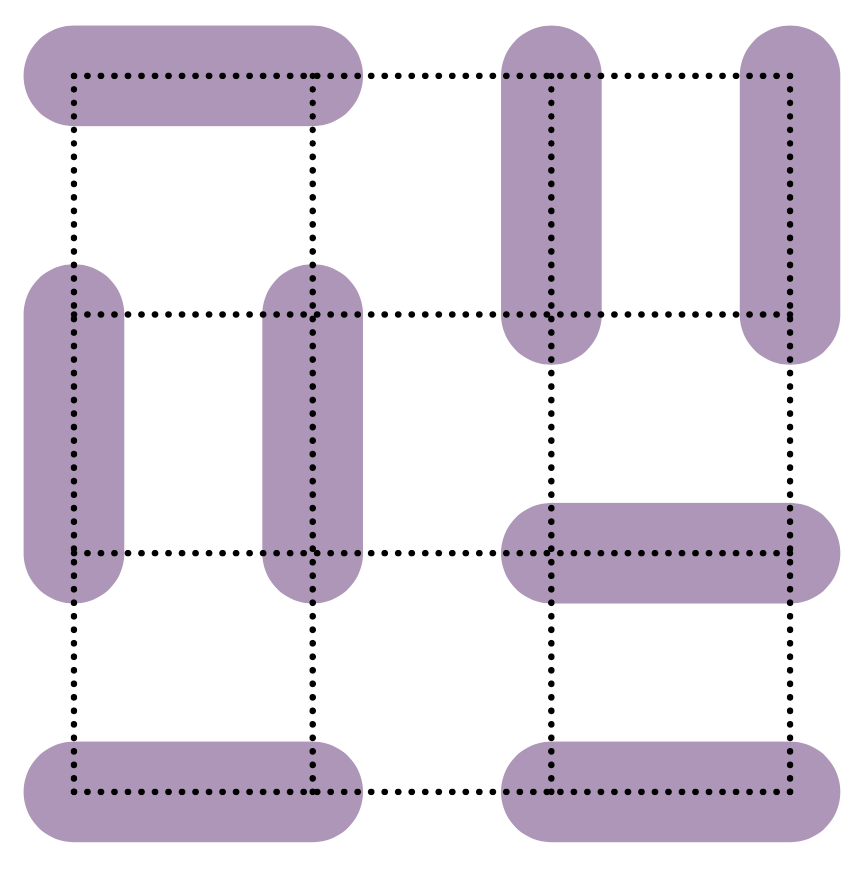
\includegraphics[width=.2\textwidth]{./images/domino_4_4.png}
	\end{equation*}
	If the set of allowed spin configurations is the 
	set of perfect matchings,
	and 
	\begin{equation*}
		H(\omega)=\begin{cases}
			0,&\textnormal{$\omega$ is a perfect matching};\\
			+\infty,&\textnormal{$\omega$ is not a perfect matching},
		\end{cases}
	\end{equation*}
	then the corresponding Gibbs measure
	is the 
	uniform distribution
	on the space of \emph{domino tilings}.
	That is, we identify each covered edge with a $2\times 1$ domino.
	The domino tiling corresponding to the above perfect matching is
	\begin{equation*}
		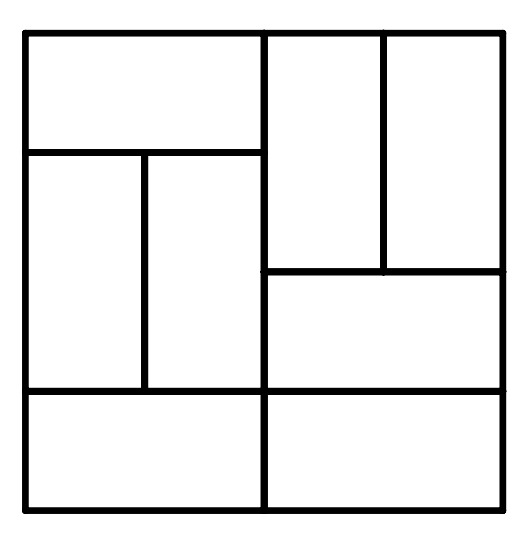
\includegraphics[width=.2\textwidth]{./images/tiling_4_4.png}
	\end{equation*}
\end{example}

Computing partition functions of various Gibbs measures
may be very nontrivial. For example, the number of 
domino tilings of the $8\times 8$ chessboard is 12,998,816,
but its theoretical computation (not via a computer program)
requires several steps. 

\colorbox{yellow}{\parbox{.7\textwidth}{ref}}

Parameter-dependent partition functions represent many important 
quantities across all of mathematics, including various
families of symmetric functions (such as Schur or Hall-Littlewood functions), and related objects.

\subsubsection{Infinite-volume Gibbs measures}


\subsubsection{Six vertex model}

\subsection{Stochastic six vertex model and its particle system limits}
\label{sub:s6v_and_degenerations}



\subsection{Gibbs properties of the stochastic six vertex model}
\label{sub:Gibbs_s6v}


\subsection{Basic coupling and colored (multispecies) models}
\label{sub:colored}

\begin{figure}[htpb]
	\centering
	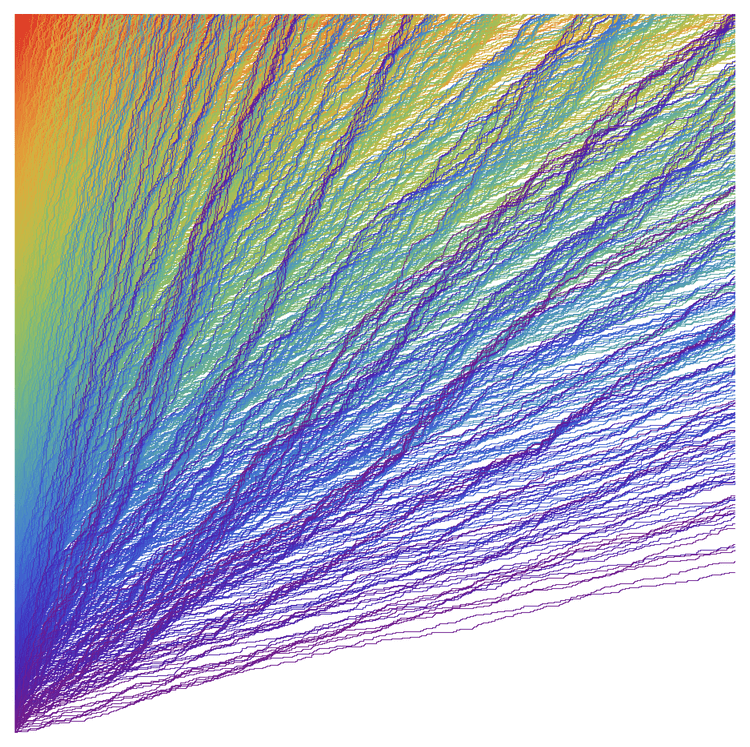
\includegraphics[width=.3\textwidth]{./images/CS6V.png}
	\quad
	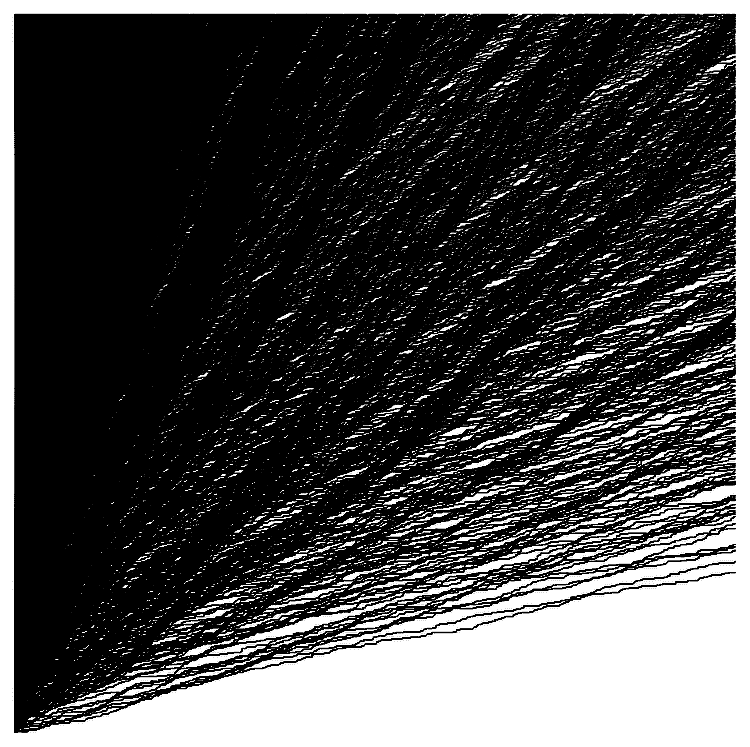
\includegraphics[width=.3\textwidth]{./images/S6V.png}
	\caption{Colored stochastic six vertex model and its monochrome version.}
	\label{fig:CS6V}
\end{figure}




\subsection{Stationary distributions and hydrodynamics}
\label{sub:hydrodynamic_analysis}





\subsection{Limit shape and fluctuation problem}
\label{sub:limit_shape_problem}










\newpage
\section{Integrability}
\label{sec:integrability}





\newpage
\section{Asymptotics}
\label{sec:asymptotics}







\newpage
\bibliographystyle{alpha}
\bibliography{bib}

\medskip

\textsc{University of Virginia, Charlottesville, VA}

E-mail: \texttt{lenia.petrov@gmail.com}


\end{document}
